%%%%%   Capitulo 3 : Diseño Conceptual    %%%%%
\chapter{Diseño Conceptual}

%%%%%   Metodología del Diseño Conceptual    %%%%%
\section{Metodología del Diseño Conceptual}
En el apartado del diseño de la solución esta presenta la fase conceptual, en donde el diseño está más enfocado en la generación y selección de conceptos de solución. Esta fase se caracteriza por tener presentar diferentes metodologías o maneras de generar alternativas, así como de evaluar estas. Algunos ejemplos de estas metodologías de generación de alternativas están presentes en el libro de \cite{dieter2012engineering}, donde explica métodos creativos como la lluvia de ideas, la sinéctica y el diseño biomimetico, así como métodos sistemáticos como la descomposición y síntesis funcional, el análisis morfológico y la teoría de la resolución inventiva de problemas (conocida como TRIZ por sus siglas en ruso). Por otro lado, en las metodologías de evaluación, \cite{dieter2012engineering} muestra los métodos sistemáticos de evaluación por medio de matrices de decisión, determinado por criterios ponderados, y en los cuales se destaca la Asignación Directa, el Árbol de Objetivos y el Proceso Analítico de Jerarquía (AHP por sus siglas en ingles).

En el marco de este proyecto se hará de la metodología sistema tanto para la generación como la evaluación de alternativas de diseño. En el parte de la generación se hará uso de la descomposición y síntesis funcional, así como del análisis morfológico; mientras que en la evaluación se hará uso del método de Asignación Directa y el AHP. Estos serán dispuestos de la siguiente manera:

\begin{enumerate} \nosep
    \item Descomposición y Síntesis Funcional.
    \item Selección de tecnología de maquina herramientas a través del método de Asignación Directa.
    \item Análisis morfológico.
    \item Generación de Alternativas.
    \item Proceso Analítico de Jerarquía  (AHP).
\end{enumerate}

%%%%%   Descomposición y Síntesis Funcional    %%%%%
\section{Descomposición y Síntesis Funcional del Sistema}
Este método de diseño conceptual, la descomposición y síntesis funcional, se basa en la estrategia común de descomponer un sistema complejo en unidades más sencillas que describan lo describan significativamente. Esta descomposición, además de ser obvia para el equipo desarrollador, debe reflejar ciertas agrupaciones naturales que comprenden una entidad o que sean mutuamente acordados por los usuarios. Por otra parte, este procedimiento es útil para comprender la tarea de diseño y asignarle recursos \citep{dieter2012engineering}. 

Basado en lo descrito por \cite{dieter2012engineering}, este método consta de 3 partes, una Descomposición Física, una Representación Funcional (o Despliegue de Funciones) y una Estructura Funcional (o Análisis Funcional).

Para este proyecto se llevará a cabo el Despliegue de Funciones (ver Sec. \ref{sec:DespliguedeFunciones}) y el Análisis Funcional (ver Sec. \ref{sec:AnalisisFuncional}).

%%%%%   Despliegue de Funciones    %%%%%
\subsection{Despliegue de Funciones}
\label{sec:DespliguedeFunciones}

El despliegue de funciones consiste de una descomposición del sistema a diseñar, partiendo desde la función global del dispositivo, pasando por cada una de las funciones que debe llevar a cabo y finalizando en las subfunciones necesarias. Con estos tres niveles funcionales se diseña el esquema del despliegue de funciones de la máquina herramienta, ver Figura \ref{fig:DespliegueFuncional}. Aparte de esto, especifican las funciones del mecanismo en la siguiente subsección. 

\begin{figure}[ht!]
    \centering
    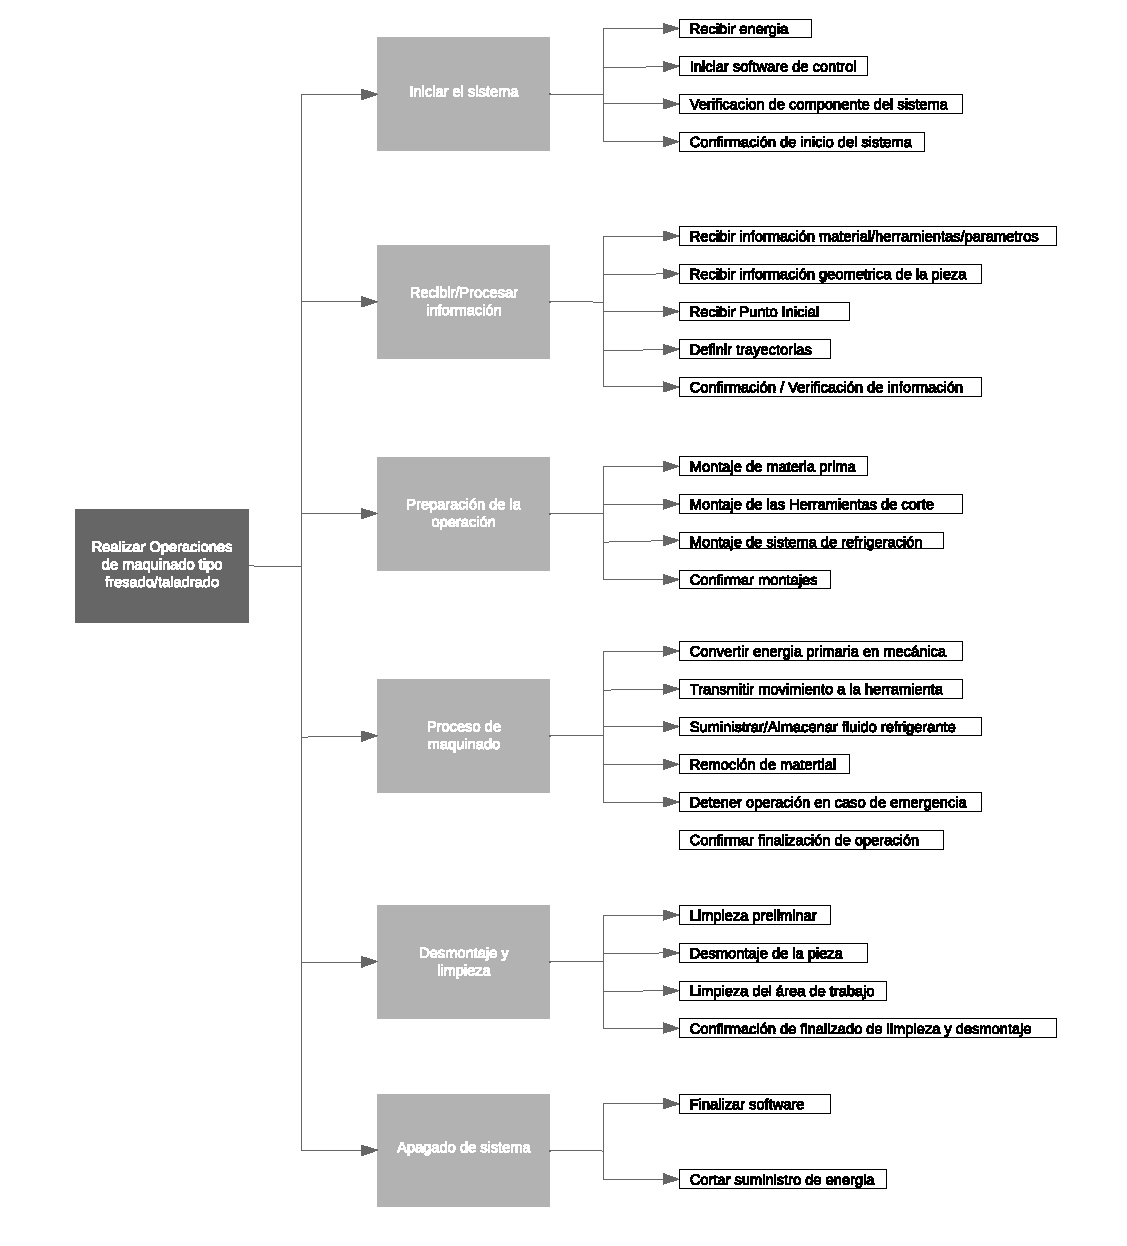
\includegraphics[width = \textwidth]{Cap3_DisenoConceptual/Figura/DespliegueFuncional.pdf}
    \caption{Despliegue de Funciones de la Máquina Herramienta}{Fuente: Elaboración Propia}
    \label{fig:DespliegueFuncional}
\end{figure}

\subsubsection{Descripción detallada de las funciones}
El buen funcionamiento de la máquina herramienta se lleva a cabo a través de las funciones presentadas a continuación:

\textbf{Iniciar el sistema}: Es necesario suministrar energía eléctrica a la máquina, de esta manera encender el sistema de control que esta posee. Al iniciar este proceso se verifican los componentes de la máquina y se recibe una confirmación por parte del sistema de control indicando que la máquina se encuentra lista para empezar a ser configurada para la operación. 

\textbf{Recibir/Procesar información}: El técnico encargado de la operación de maquinado se encargará de suministrar la información sobre el material, herramientas de corte y parámetros de la operación. así mismo el técnico suministra lo geometría de la pieza de trabajo (geometría inicial y final). Es necesario que antes de la operación tener un punto cero de referencia. Teniendo ya los datos anteriores el software definirá las trayectorias y velocidades a las que se realizarán los cortes. El software confirmara que todos los parámetros estén bien definidos y mostrará un resumen de operación para que el técnico de pueda dar inicio a la operación.

\textbf{Preparar operación de maquinado}: Una vez el operario haya iniciado el sistema procederá a realizar el montaje de la materia prima con la que se realizará el trabajo, así como el montaje de la herramienta de corte idónea para los resultados y/o requerimientos finales de la pieza a fabricar.  En estos procesos de maquinado donde el desbaste de material genera una cantidad de calor considerable resulta importante contar con un sistema de refrigeración el cual será montado por el operario. Para finalizar y garantizar el buen funcionamiento el operario debe confirmar los montajes realizados.

\textbf{Iniciar proceso de maquinado}:  Una vez finalizadas las funciones previas, la máquina debe transformar la energía eléctrica a energía mecánica para comenzar con el movimiento de los elementos de la máquina. Partiendo del movimiento de los actuadores se debe transmitir el movimiento a la herramienta, teniendo en cuenta las potencias requeridas. En este punto la máquina-herramienta se encuentra lista para empezar con la remoción de material. Hasta el final del proceso de remoción de material la máquina debe suministrar fluido de refrigeración a la zona en herramienta pieza que se encuentran en operación. En caso de alguna emergencia o mal funcionamiento se debe poder detener la operación. Si todo el procedimiento se lleva a cabo de manera adecuada se recibirá una confirmación de finalización de la operación. 

\textbf{Desmontar y limpiar pieza y área de trabajo}: Después de que la operación de maquinado haya finalizado, la máquina comenzará una limpieza preliminar con un chorro de aire para retirar la viruta de la superficie de la pieza maquinada. Después el técnico encargado retirar la pieza de trabajo y dar inicio a la limpieza del área de trabajo.

\textbf{Apagar de sistema}: Una vez finalizado todo es proceso de mecanizado y limpieza, sabiendo que no se hará otra operación de maquinado el técnico que opera la máquina apagará el software y quitará el fluido eléctrico de la máquina.

%%%%%   Análisis Funcional    %%%%%
\subsection{Análisis Funcional}
\label{sec:AnalisisFuncional}

El análisis funcional busca producir un diagrama de bloques, que represente los flujos de energía, material, y señal (o información) como flechas etiquetadas tomando un camino entre los bloques de funciones. El análisis funcional más general consta de un simple bloque de función, la cual describe la función global del dispositivo; este diagrama se conoce como \enquote{caja negra} y es un punto de partida pare el diseño de nuevos equipos o dispositivos. Luego de esto, y con ayuda de lo encontrado en el despliegue de funciones, es posible generar un diagrama que interrelacione todas las subfunciones del producto, así como los flujos que conectan a estas; este nuevo diagrama se le conoce como \enquote{Caja transparente} \citep{dieter2012engineering}.

Los diagramas obtenidos para este proyecto se pueden observar en las figuras \ref{fig:CajaNegra} y \ref{fig:CajaTransparente}.

\begin{figure}[htb!]
    \centering
    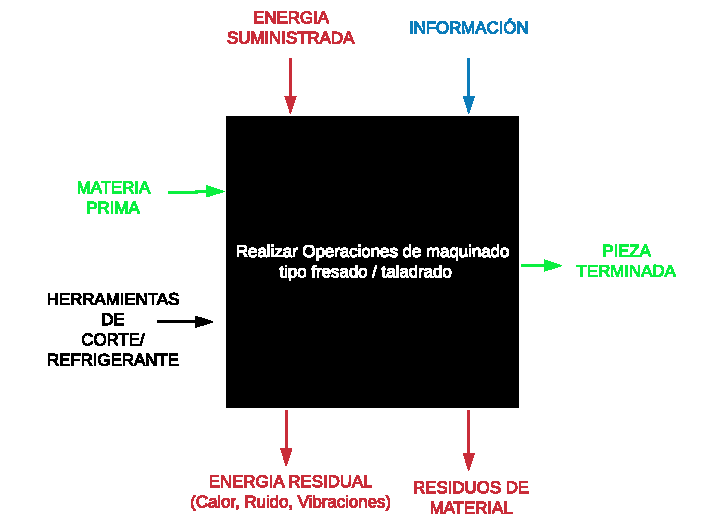
\includegraphics[width = 0.5 \textwidth]{Cap3_DisenoConceptual/Figura/CajaNegra.pdf}
    \caption{Caja Negra de la Máquina Herramienta}{Fuente: Elaboración Propia}
    \label{fig:CajaNegra}
\end{figure}

\begin{figure}[htb!]
    \centering
    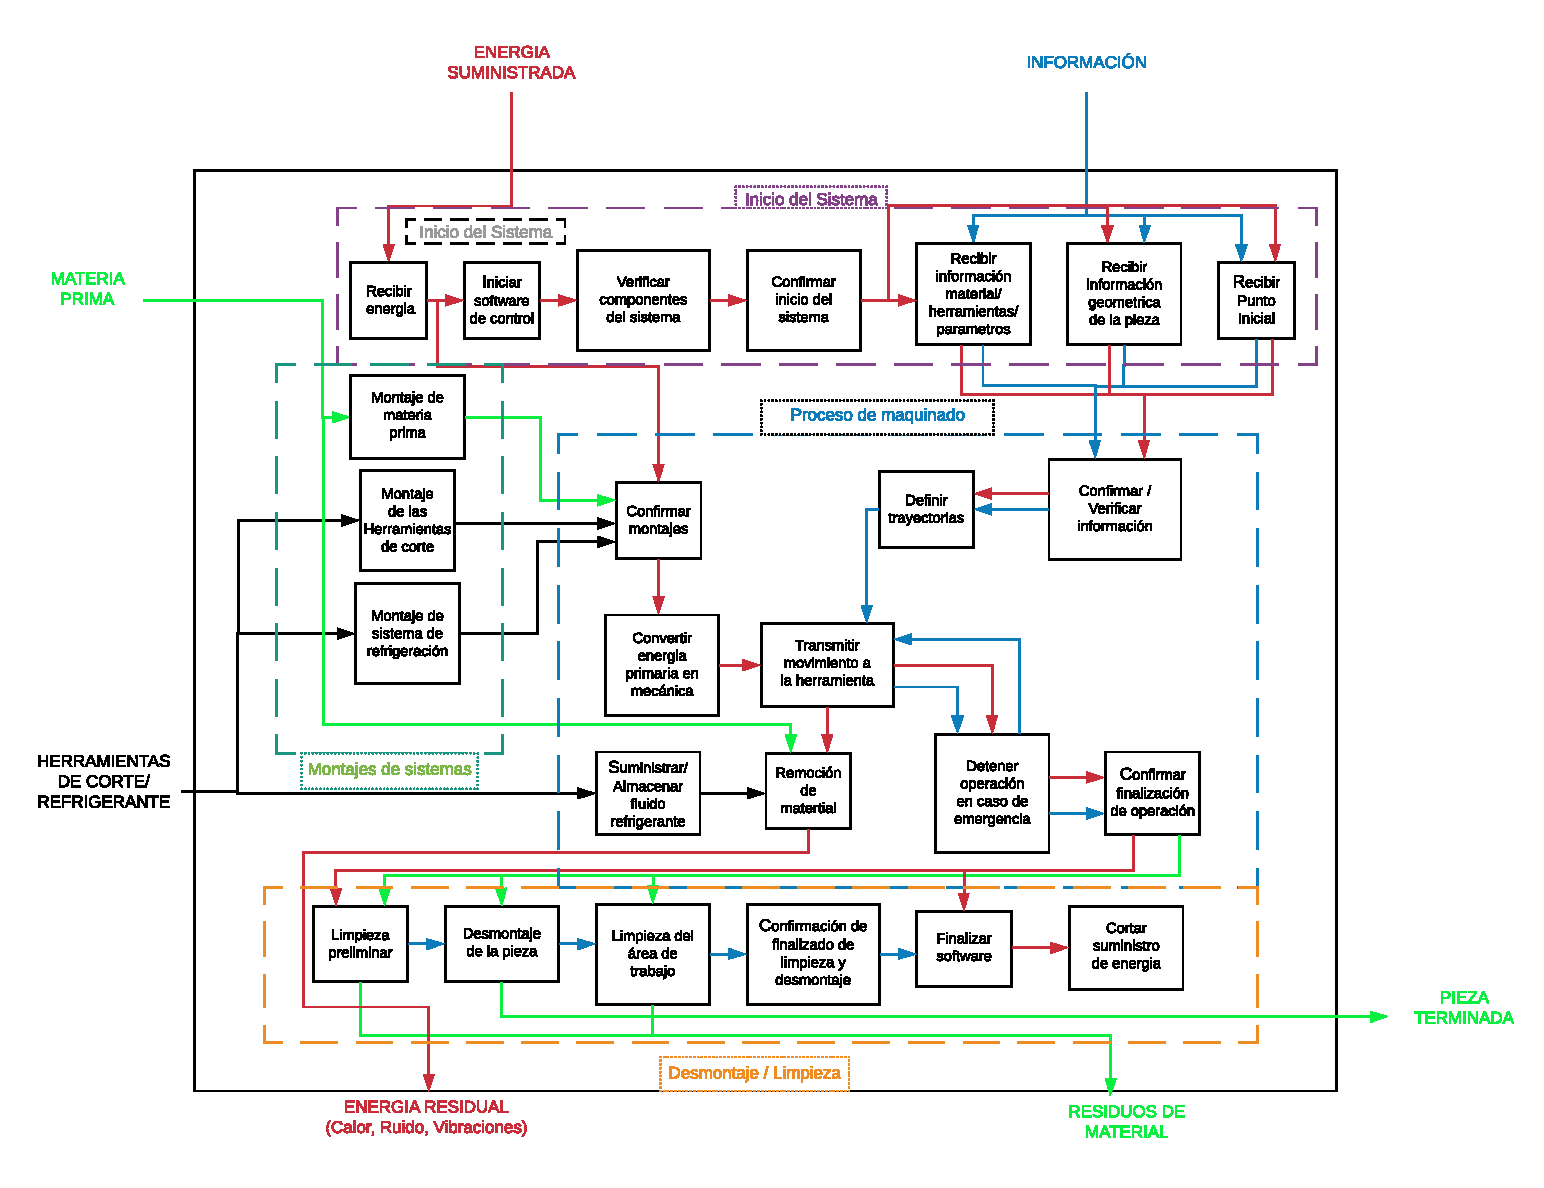
\includegraphics[width= \textwidth]{Cap3_DisenoConceptual/Figura/CajaTransparente.pdf}
    \caption{Caja Transparente de la Máquina Herramienta}{Fuente: Elaboración Propia}
    \label{fig:CajaTransparente}
\end{figure}

%%%%%   Selección de la tecnología de Máquina Herramienta    %%%%%
\section{Selección de la tecnología de Robot Herramienta}
Para la selección de tecnología  

\begin{longtable}{|>{\columncolor[gray]{0.85}} p{0.25\textwidth}| c | c   c   c |}
    \hline \rowcolor[gray]{0.85}
     & \rotatebox{90}{\textbf{Importancia}} & \rotatebox{90}{\textbf{Convencional~}} & \rotatebox{90}{\textbf{Serial}} & \rotatebox{90}{\textbf{Paralela}} \\ \hline \endhead
    Costo de Adquisición & 20 & 10 &  5 &  7\\ \hline
    Costo Mantenimiento  & 10 &  9 &  7 &  5\\ \hline
    Precision/Rigidez    & 20 &  8 &  5 & 10\\ \hline
    Seguridad            &  5 &  8 &  7 &  9\\ \hline
    Compacidad           &  5 &  6 & 10 &  7\\ \hline
    Modularidad          & 10 &  7 &  7 & 10\\ \hline
    Control              &  5 & 10 &  8 &  6\\ \hline
    Capacidad de carga   & 15 &  7 &  5 &  9\\ \hline
     & 100 & \textbf{36.38} & 26.34 & \textbf{37.28} \\ \hline
    \caption{Selección de Tecnología }{Fuente: Elaboración Propia}
    \label{table:SeleccionTecnologia}
\end{longtable}

\section{Análisis morfológico}

\small
\begin{longtable}{| >{\columncolor[gray]{0.85}} c | >{\columncolor[gray]{0.85}} c | >{\columncolor[gray]{0.85}} p{0.2\textwidth} | p{0.15\textwidth}   p{0.15\textwidth}   p{0.15\textwidth} |}

\hline \rowcolor[gray]{0.85}
 Función & N & Subfunción                               & Concepto de solución 1      & Concepto de solución 2   & Concepto de solución 3 \\ \hline \endhead
 & 1 & Tipo de alimentación de energía          & Electrica                     & Hidraulica & Neumatica \\ \cline{2-6}
 & 2 & Transmitir energía hacia los componentes & Conexiones eléctrica        & Tuberia hidraulica  & Tuberia Neumatica \\ \cline{2-6}
 & 3 & Sistema de control                       & Computarizado               & Manual                   & Semiautomático\\ \cline{2-6}
\multirow{-4}{*}{ Iniciar Sistema}& 4 & Software                                 & Arduino                     & Python                   & LabVIEW\\ \hline
 
 &  5 & Montaje de herramienta de corte          & Acople magnético            & Acople tipo mordaza      &\\  \cline{2-6}
 &  6 & Sujeción de materia prima                & Mordazas mecánicas          & Mordazas hidráulicas       & Mordazas neumáticas  \\ \cline{2-6}
\multirow{-3}{*}{Preparar Montajes} &  7 & Sistema de refrigeración                 & Refrigeración por aire      & Refrigeración por liquido & Refrigeración Mixto\\ \cline{1-6}
 &  8 & Cinemática                               & Convencional                & Paralela (Try-Piramid)    & Paralela (UPU)\\ \cline{2-6}

 & 9 & Actuadores                               & Motor paso a paso           & Motores síncronos	       & \\ \cline{2-6}
 & 10 & Sistema de guiado                        & Rieles                      & Ejes                     & Cable\\ \cline{2-6}

 
 & 11 & Sistema de transmisión de movimiento     & Tornillo de potencia        & Cilindro-pistón           & Transmisión por correa\\ \cline{2-6}
 \multirow{-4}{*}{ Mecanizar} & 12 & Sistema de parada de emergencia          & Sistema mecánico bloqueante & Sistema corta corriente   & \\ \hline

 & 13 & Sistema de limpieza                      & Aire comprimido             & Agua a presión            & Barrido manual\\ \cline{2-6}
  \multirow{-2}{*}{ Finalizar operación} & 14 & Confirmar finalización de operación      & Indicador led               & Indicador digital         & Indicador sonoro \\ \hline

\caption{Diagrama Morfológico}
\label{table:DiagramaMorfologico}
\end{longtable}

\section{Generación de Alternativas}

\section{Proceso Analítico de Jerarquía  (AHP)}